\documentclass[tikz,border=10pt]{standalone}
\begin{document}
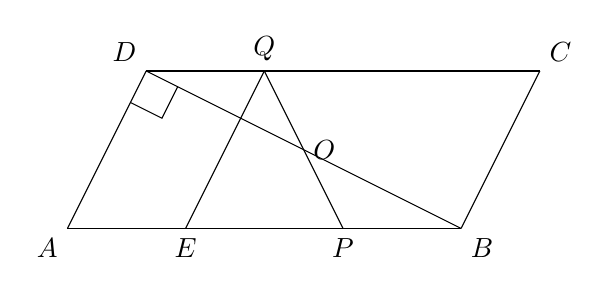
\begin{tikzpicture}
    \coordinate (A) at (0,0);
    \coordinate (B) at (5,0);
    \coordinate (C) at (6,2);
    \coordinate (D) at (1,2);
    \coordinate (E) at (1.5,0);
    \coordinate (P) at (3.5,0);
    \coordinate (Q) at (2.5,2);
    \coordinate (O) at (3,1);

    % Draw the parallelogram sides
    \draw (A) -- (B);
    \draw (B) -- (C);
    \draw (C) -- (D);
    \draw (D) -- (A);
    
    % Draw internal lines
    \draw (D) -- (B);
    \draw (Q) -- (E);
    \draw (Q) -- (P);
    
    % Right angle mark at D between AD and DB
    % Vector DA is approx (-1, -2), Vector DB is approx (4, -2) which is parallel to (2, -1)
    % We construct a small square corner
    \coordinate (D1) at (0.8, 1.6); 
    \coordinate (D2) at (1.4, 1.8); 
    \coordinate (D3) at (1.2, 1.4); 
    \draw (D1) -- (D3) -- (D2);
    
    % Labels
    \node[below left] at (A) {$A$};
    \node[below right] at (B) {$B$};
    \node[above right] at (C) {$C$};
    \node[above left] at (D) {$D$};
    \node[below] at (E) {$E$};
    \node[below] at (P) {$P$};
    \node[above] at (Q) {$Q$};
    \node[right] at (O) {$O$};
\end{tikzpicture}
\end{document}
